\documentclass{math}

\usepackage{tikz}

\title{University Physics 2}
\author{Alvin Lin}
\date{January 2018 - May 2018}

\begin{document}

\maketitle

\section*{Magnetic Fields}
The magnetic force on a particle is given as:
\[ \overrightarrow{F_B} = q(\vec{V}\times\vec{B}) \]
Note that the force requires the charge to be moving and is perpendicular to
both the velocity and the field since it is a cross product. Using the
properties of cross products, we can express this as:
\[ |\overrightarrow{F_B}| = q|\vec{V}||\vec{B}|\sin\theta \]

\subsubsection*{Cross Products}
Recall the following properties of cross products:
\begin{enumerate}
  \item Magnitude is a function of the vector magnitudes and the sine of the
  angle between them.
  \[ |\vec{A}\times\vec{B}| = |\vec{A}||\vec{B}|\sin\theta \]
  \item Direction follows the right-hand rule. Put your fingers in the direction
  of A, curl your fingers towards B, and your thumb will point towards C. With
  respect to its application to magnetic fields, we put our fingers in the
  direction of \( \vec{V} \), curl them towards \( \vec{B} \), and our thumb
  will point towards \( \overrightarrow{F_B} \).
  \item Using unit vectors:
  \begin{align*}
    \i\times\j &= \k \quad \i\times\k = -\j \\
    \j\times\k &= \i \quad \k\times\j = -\i \\
    \k\times\i &= \j \quad \j\times\i = -\k
  \end{align*}
\end{enumerate}

\subsection*{Lorentz Force Law}
Recall the following from electric fields:
\[ \vec{F} = q\vec{E} \]
Thus, the net force of an electric and magnetic field is:
\begin{align*}
  \vec{F} &= \overrightarrow{F_E}+\overrightarrow{F_B} \\
  &= q\vec{E}+q(\vec{V}\times\vec{B}) \\
  &= q(\vec{E}+\vec{V}\times\vec{B})
\end{align*}
If we're dealing with magnetic fields only:
\begin{align*}
  \overrightarrow{F_B} &= q(\vec{V}\times\vec{B}) \\
  |\overrightarrow{F_B}| &= q|\vec{V}||\vec{B}|\sin\theta \\
  If: \theta &= 90 \\
  |\overrightarrow{F_B}| &= q|\vec{V}||\vec{B}|
\end{align*}
By the properties of cross products, we know that \( \overrightarrow{F_B} \) is
perpendicular to both \( \vec{V} \) and \( \vec{B} \). Recall that work
\( W = \vec{F}\cdot\delta\vec{r} \) is a dot product. Since \( \Delta\vec{r} \)
will be in the same direction as \( \vec{V} \),
\( \overrightarrow{F_B}\cdot\Delta\vec{r} = 0 \). Therefore, magnetic fields do
no work.

\subsection*{Lorentz Force Law for a Wire}
Moving charge is current, recall that:
\[ I = nq|\vec{V}|A \]
where \( n \) is charge density. The total number of charges in the wire
is calculated as \( nAL \) where \( A \) is the cross-sectional area of the wire
and \( L \) is the length of the wire. If the force on one charge passing
through the wire is \( |\vec{F}| = q|\vec{V}||\vec{B}| \), then the total force
on all the charges passing through the wire  is equal to:
\begin{align*}
  |\vec{F_B}| &= (nAL)(q|\vec{V}||\vec{B}|) \\
  &= (nq|\vec{V}|A)(L|\vec{B}|) \\
  &= IL|\vec{B}| \\
  \vec{F_B} &= I\vec{L}\times\vec{B}
\end{align*}
where \( \vec{L} \) is a vector with the length of the wire, pointing in the
direction of current. This is only true if the magnetic field is constant over
the length of the wire. Otherwise, integration is necessary in order to
calculate \( \vec{F_B} \).

\subsubsection*{Example}
What is the net force on the following loop of wire?
\begin{center}
  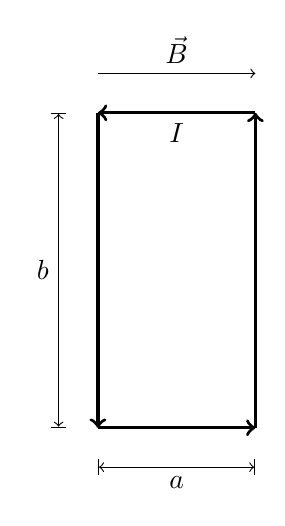
\begin{tikzpicture}
    \draw[very thick,->] (1,2) -- (-1,2) node[below,pos=0.5] {\( I \)};
    \draw[very thick,->] (-1,2) -- (-1,-2);
    \draw[very thick,->] (-1,-2) -- (1,-2);
    \draw[very thick,->] (1,-2) -- (1,2);
    \draw[->] (-1,2.5) -- (1,2.5) node[above,pos=0.5] {\( \vec{B} \)};
    \draw[|<->|] (-1,-2.5) -- (1,-2.5) node[below,pos=0.5] {\( a \)};
    \draw[|<->|] (-1.5,-2) -- (-1.5,2) node[left,pos=0.5] {\( b \)};
  \end{tikzpicture}
\end{center}
\begin{align*}
  \vec{F} &= I\vec{L}\times\vec{B} \\
  \overrightarrow{F_{top}} &= \overrightarrow{F_{bottom}} = \vec{0} \\
  \overrightarrow{F_{total}} &= \overrightarrow{F_{top}}+
    \overrightarrow{F_{bottom}}+\overrightarrow{F_{left}}+
    \overrightarrow{F_{right}} \\
  &= IbB\k+IbB(-\k) \\
  &= 0
\end{align*}
Note that the net force from the magnetic field is zero, but there is a net
torque exerted on the loop of wire.
\begin{align*}
  \vec{\tau} &= \vec{r}\times\vec{F} \\
  \overrightarrow{\tau_{top}} &= \overrightarrow{\tau_{bottom}} = \vec{0} \\
  \overrightarrow{\tau_{total}} &= \overrightarrow{\tau_{top}}+
    \overrightarrow{\tau_{bottom}}+ \overrightarrow{\tau_{left}}+
    \overrightarrow{\tau_{right}} \\
  &= \frac{a}{2}IbB\j+\frac{a}{2}IbB\j \\
  &= IabB\j \\
  &= IAB\j
\end{align*}
where \( A \) is the area enclosed by the loop of wire. Note that \( \mu = IA \)
is known as the magnetic dipole moment.

\subsection*{Electric and Magnetic Dipoles}
Recall from electric dipoles that the dipole moment points from the negative
charge to the positive charge and has a magnitude of \( qd \). We calculate
torque for an electric dipole as \( \overrightarrow{\tau_E} =
\vec{p}\times\vec{E} \). For magnetic dipoles, an analogous concept applies.
The torque on a magnetic dipole is \( \overrightarrow{\tau_B} =
\vec{\mu}\times\vec{B} \).

\subsection*{Magnetic Field Creation}
Magnetic fields all arise from current loops. Atoms are current loops as well.
In physical materials, these current loops are evenly distributed and cancel
out. For magnets, these current loops are aligned, creating a stronger magnetic
field. An atom is the simplest current loop and the simply way to generate an
magnetic field. Electric monopole can exists which propagate an electric field
outwards in all direction. No analogous magnetic monopole exists since magnetic
field lines always close on themselves. Magnetic fields are created by moving
charge and defined as follows:
\[ \vec{B} = \frac{\mu_{\circ}}{4\pi}\frac{q\vec{V}\times\vec{r}}{r^2} \]
where \( \mu_{\circ} \) is the magnetic constant, \( q \) is the charge,
\( \vec{V} \) is the speed of the charge, \( r \) is the distance from the point
of observation, and \( \vec{r} \) is a unit vector pointing from the charge to
the point of observation. Note that this formula for a magnetic field is
analogous that of an electric field.

\subsection*{Biot-Savart Law}
Current is just a bunch of moving charges in a wire, so magnetic fields are
generated by current moving through a wire.
\begin{center}
  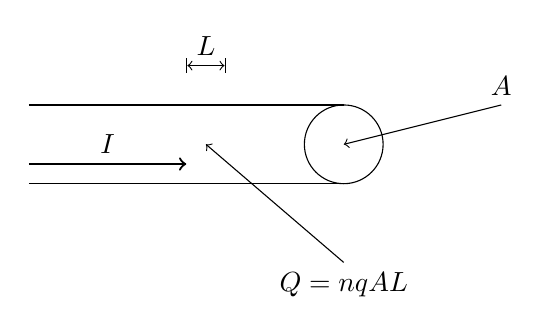
\begin{tikzpicture}
    \draw (-2,0) -- (2,0);
    \draw (-2,1) -- (2,1);
    \draw (2,0.5) circle (0.5cm);
    \draw[|<->|] (0,1.5) -- (0.5,1.5) node[above,pos=0.5] {\( \diff{L} \)};
    \draw[->] (2,-1) -- (0.25,0.5) node[below,pos=0]
      {\( \diff{Q} = nqA\diff{L}\)};
    \draw[->,thick] (-2,0.25) -- (0,0.25) node[above,pos=0.5] {\( I \)};
    \draw[->] (4,1) -- (2,0.5) node[pos=0,above] {\( A \)};
  \end{tikzpicture}
\end{center}
\begin{align*}
  I &= nqA\vec{V} \\
  \diff{\vec{B}} &=
    \frac{\mu_{\circ}}{4\pi}\frac{\diff{Q}\vec{V}\times\vec{r}}{r^2} \\
  &= \frac{\mu_{\circ}}{4\pi}nqA\diff{\vec{L}}
    \frac{\vec{V}\times\vec{r}}{r^2} \\
  &= \frac{\mu_{\circ}}{4\pi}(nqA\vec{V})
    \frac{\diff{\vec{L}}\times\vec{r}}{r^2} \\
  &= \frac{\mu_{\circ}I}{4\pi}\frac{\diff{\vec{L}}\times\vec{r}}{r^2} \\
  \vec{B} &= \frac{\mu_{\circ}}{4\pi}
    \int I\frac{\diff{\vec{L}}\times\vec{r}}{r^2}
\end{align*}
This relation is known as the Biot-Savart Law. All directions of magnetic fields
come from using the right hand rule on the Biot-Savart Law where the
fingers point in the direction of \( \diff{\vec{s}} \) and are curled in the
direction of \( \vec{r} \), thus pointing in the direction of
\( \diff{\vec{B}} \).

\subsection*{Ampere's Law}
\[ \oint\vec{B}\cdot\diff{\vec{s}} = \mu_{\circ}I_{enc} \]
Suppose we have a wire with current coming out of the page.
\begin{center}
  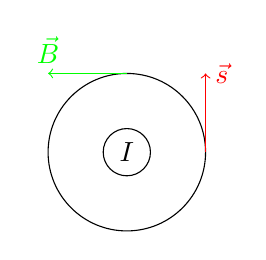
\begin{tikzpicture}
    \draw (0,0) circle (0.3cm) node {\( I \)};
    \draw (0,0) circle (1cm);
    \draw[->,red] (1,0) -- (1,1) node[right] {\( \diff{\vec{s}} \)};
    \draw[->,green] (0,1) -- (-1,1) node[above] {\( \vec{B} \)};
  \end{tikzpicture}
\end{center}
Ampere's Law is applied very similarly to Gauss's Law.
\[ \oint\vec{B}\cdot\diff{\vec{s}} = \int B\diff{s} = B\int\diff{s} = B2\pi r \]
This simplification can be made because of circular symmetry and because the
magnetic field \( \vec{B} \) is parallel to \( \diff{\vec{s}} \) around the
wire.

\begin{center}
  You can find all my notes at \url{http://omgimanerd.tech/notes}. If you have
  any questions, comments, or concerns, please contact me at
  alvin@omgimanerd.tech
\end{center}

\end{document}
